 %package list
\documentclass{article}
\usepackage[top=3cm, bottom=3cm, outer=3cm, inner=3cm]{geometry}
\usepackage{multicol}
\UseRawInputEncoding
\usepackage{graphicx}
\usepackage{url}
%\usepackage{cite}
\usepackage{hyperref}
\usepackage{array}
%\usepackage{multicol}
\newcolumntype{x}[1]{>{\centering\arraybackslash\hspace{0pt}}p{#1}}
\usepackage{natbib}
\usepackage{pdfpages}
\usepackage{multirow}
\usepackage[normalem]{ulem}
\useunder{\uline}{\ul}{}
\usepackage{svg}
\usepackage{xcolor}
\usepackage{listings}
\lstdefinestyle{ascii-tree}{
    literate={├}{|}1 {─}{--}1 {└}{+}1
  }
\lstset{basicstyle=\ttfamily,
  showstringspaces=false,
  commentstyle=\color{red},
  keywordstyle=\color{blue}
}
%\usepackage{booktabs}
\usepackage{caption}
\usepackage{subcaption}
\usepackage{float}
\usepackage{array}

\newcolumntype{M}[1]{>{\centering\arraybackslash}m{#1}}
\newcolumntype{N}{@{}m{0pt}@{}}

%------------------------------ ÍTEMS --------------------------------

\newcommand{\itemEmail}{hchoquehuancaz@unsa.edu.pe}
\newcommand{\itemStudent}{Hernan Andy Choquehuanca Zapana}
\newcommand{\itemCourse}{Fundamentos de la Programacion II}
\newcommand{\itemCourseCode}{1701213}
\newcommand{\itemSemester}{II}
\newcommand{\itemUniversity}{Universidad Nacional de San Agustin de Arequipa}
\newcommand{\itemFaculty}{Facultad de Ingenieria de Produccion y Servicios}
\newcommand{\itemDepartment}{Departamento Academico de Ingenieria de Sistemas e Informatica}
\newcommand{\itemSchool}{Escuela Profesional de Ingenieria de Sistemas}
\newcommand{\itemAcademic}{2023 - B}
    \newcommand{\itemInput}{Del 08 Enero 2024}
\newcommand{\itemOutput}{Al 10 Enero 2024}
\newcommand{\itemPracticeNumber}{20}
\newcommand{\itemTheme}{Definici\'on de Clases de Usuario, Herencia y Polimorfismo.}

%------------------------------  ------------------------------

\usepackage[english,spanish]{babel}
\usepackage[utf8]{inputenc}
\AtBeginDocument{\selectlanguage{Spanish}}
\renewcommand{\figurename}{Figura}
\renewcommand{\refname}{Referencias}
\renewcommand{\tablename}{Tabla} %esto no funciona cuando se usa babel
\AtBeginDocument{
	\renewcommand\tablename{Tabla}
}

\usepackage{fancyhdr}
\pagestyle{fancy}
\fancyhf{}
\setlength{\headheight}{30pt}
\renewcommand{\headrulewidth}{1pt}
\renewcommand{\footrulewidth}{1pt}
\fancyhead[L]{\raisebox{-0.2\height}{
\includegraphics[width=3cm]{img/logo_episunsa.png}}}
\fancyhead[C]{\fontsize{7}{7}\selectfont	\itemUniversity \\ \itemFaculty \\ \itemDepartment \\ \itemSchool \\ \textbf{\itemCourse}}
\fancyhead[R]{\raisebox{-0.2\height}{
\includegraphics[width=1.2cm]{img/logo_abet}}}
\fancyfoot[L]{Estudiante: Hernan Choquehuanca Zapana}
\fancyfoot[R]{\itemCourse}
\fancyfoot[C]{Página \thepage}

% para el codigo fuente
\usepackage{listings}
\usepackage{color, colortbl}
\definecolor{dkgreen}{rgb}{0,0.6,0}
\definecolor{gray}{rgb}{0.5,0.5,0.5}
\definecolor{mauve}{rgb}{0.58,0,0.82}
\definecolor{codebackground}{rgb}{0.95, 0.95, 0.92}
\definecolor{tablebackground}{rgb}{0.8, 0, 0}

\lstset{frame=tb,
	language=bash,
	aboveskip=3mm,
	belowskip=3mm,
	showstringspaces=false,
	columns=flexible,
	basicstyle={\small\ttfamily},
	numbers=none,
	numberstyle=\tiny\color{gray},
	keywordstyle=\color{blue},
	commentstyle=\color{dkgreen},
	stringstyle=\color{mauve},
	breaklines=true,
	breakatwhitespace=true,
	tabsize=3,
	backgroundcolor= \color{codebackground},
}

%------------------------------ INICIO DEL DOCUMENTO------------------------------

\begin{document}
	
	\vspace*{10px}
	
	\begin{center}	
		\fontsize{17}{17} \textbf{ Informe de Laboratorio \itemPracticeNumber}
	\end{center}
	\centerline{\textbf{\Large Tema: \itemTheme}}
	%\vspace*{0.5cm}	

	\begin{flushright}
		\begin{tabular}{|M{2.5cm}|N|}
			\hline 
			\rowcolor{tablebackground}
			\color{white} \textbf{Nota}  \\
			\hline 
			     \\[30pt]
			\hline 			
		\end{tabular}
	\end{flushright}	

	\begin{table}[H]
		\begin{tabular}{|x{4.7cm}|x{4.8cm}|x{4.8cm}|}
			\hline 
			\rowcolor{tablebackground}
			\color{white} \textbf{Estudiante} & \color{white}\textbf{Escuela}  & \color{white}\textbf{Asignatura}   \\
			\hline 
			{\itemStudent \par \itemEmail} & \itemSchool & {\itemCourse \par Semestre: \itemSemester \par Código: \itemCourseCode}     \\
			\hline 			
		\end{tabular}
	\end{table}		
	
	\begin{table}[H]
		\begin{tabular}{|x{4.7cm}|x{4.8cm}|x{4.8cm}|}
			\hline 
			\rowcolor{tablebackground}
			\color{white}\textbf{Laboratorio} & \color{white}\textbf{Tema}  & \color{white}\textbf{Duración}   \\
			\hline 
			\itemPracticeNumber & \itemTheme & 10 horas   \\
			\hline 
		\end{tabular}
	\end{table}
	
	\begin{table}[H]
		\begin{tabular}{|x{4.7cm}|x{4.8cm}|x{4.8cm}|}
			\hline 
			\rowcolor{tablebackground}
			\color{white}\textbf{Semestre académico} & \color{white}\textbf{Fecha de inicio}  & \color{white}\textbf{Fecha de entrega}   \\
			\hline 
			\itemAcademic & \itemInput &  \itemOutput  \\
			\hline 
		\end{tabular}
	\end{table}


%------------------------------ ACTIVIDADES (TAREA) ------------------------------

	\section{Tarea}
	\begin{itemize}		
        \item Crear diagrama de clases UML y programa.
        \item Crear los miembros de cada clase de la forma más adecuada: como miembros de clase o de instancia.
        \item Crear la clase Mapa, que esté constituida por el tablero antes visto, que posicione soldados en ciertas posiciones aleatorias (entre 1 y 10 soldados por cada ejército, sólo 1 ejército por reino). Se deben generar ejércitos de 2 reinos. No se admite guerra civil. El Mapa tiene como atributo el tipo de territorio que es (bosque, campo abierto, montaña, desierto, playa). La cantidad de soldados, así como todos sus atributos se deben generar aleatoriamente.
        \item Dibujar el Mapa con las restricciones que sólo 1 soldado como máximo en cada cuadrado.
        \item El mapa tiene un solo tipo de territorio.
        \item Considerar que el territorio influye en los resultados de las batallas, así cada reino tiene bonus según el territorio: Inglaterra->bosque, Francia->campo abierto, Castilla-Aragón->montaña, Moros->desierto, Sacro Imperio Romano-Germánico->bosque, playa, campo abierto. En dichos casos, se aumenta el nivel de vida en 1 a todos los soldados del reino beneficiado.
        \item En la historia, los ejércitos estaban conformados por diferentes tipos de soldados, que tenían similitudes, pero también particularidades.
        \item Basándose en la clase Soldado crear las clases Espadachín, Arquero, Caballero y Lancero. Las cuatro clases heredan de la superclase Soldado pero aumentan atributos y métodos, o sobrescriben métodos heredados.
        \item Los espadachines tienen como atributo particular "longitud de espada" y como acción "crear un muro de escudos" que es un tipo de defensa en particular.
        \item Los caballeros pueden alternar sus armas entre espada y lanza, además de desmontar (sólo se realiza cuando está montando e implica defender y cambiar de arma a espada), montar (sólo se realiza cuando está desmontado e implica montar, cambiar de arma a lanza y envestir). El caballero también puede envestir, ya sea montando o desmontando, cuando es desmontado equivale a atacar 2 veces pero cuando está montando implica a atacar 3 veces.
        \item Los arqueros tienen un número de flechas disponibles las cuales pueden dispararse y se gastan cuando se hace eso.
        \item Los lanceros tienen como atributo particular, "longitud de lanza" y como acción "schiltrom" (como una falange que es un tipo de defensa en particular y que aumenta su nivel de defensa en 1).
        \item Tendrá 2 Ejércitos que pueden ser constituidos sólo por espadachines, caballeros, arqueros y lanceros. No se acepta guerra civil. Crear una estructura de datos conveniente para el tablero. Los soldados del primer ejército se almacenarán en un arreglo estándar y los soldados del segundo ejército se almacenarán en un ArrayList. Cada soldado tendrá un nombre autogenerado: Espadachin0X1, Arquero1X1, Caballero2X2, etc., un valor de nivel de vida autogenerado aleatoriamente, la fila y columna también autogenerados aleatoriamente (no puede haber 2 soldados en el mismo cuadrado) y valores autogenerados para el resto de atributos.
        \item Todos los caballeros tendrán los siguientes valores: ataque 13, defensa 7, nivel de vida [10..12] (el nivel de vida actual empieza con el valor del nivel de vida).
        \item Todos los arqueros tendrán los siguientes valores: ataque 7, defensa 3, nivel de vida [3..5] (el nivel de vida actual empieza con el valor del nivel de vida).
        \item Todos los espadachines tendrán los siguientes valores: ataque 10, defensa 8, nivel de vida [8..10] (el nivel de vida actual empieza con el valor del nivel de vida).
        \item Todos los lanceros tendrán los siguientes valores: ataque 5, defensa 10, nivel de vida [5..8] (el nivel de vida actual empieza con el valor del nivel de vida).
        \item Mostrar el tablero, distinguiendo los ejércitos y los tipos de soldados creados. Además, se debe mostrar todos los datos de todos los soldados creados para ambos ejércitos. Además de los datos del soldado con mayor vida de cada ejército, el promedio de nivel de vida de todos los soldados creados por ejército, los datos de todos los soldados por ejército en el orden que fueron creados y un ranking de poder de todos los soldados creados por ejército (del que tiene más nivel de vida al que tiene menos) usando algún algoritmo de ordenamiento.
        \item Finalmente, que muestre el resumen los 2 ejércitos, indicando el reino, cantidad de unidades, distribución del ejército según las unidades, nivel de vida total del ejército y qué ejército ganó la batalla (usar la métrica de suma de niveles de vida y porcentajes de probabilidad de victoria basado en ella). Este porcentaje también debe mostrarse.
        \item Hacerlo programa iterativo.
	\end{itemize}
		
\section{Equipos, materiales y temas utilizados}
	\begin{itemize}
		\item Sistema Operativo Windows 11 Pro 22H2 64 bits.
		\item Visual Studio Code.
		\item Git 2.42.0.
		\item Cuenta en GitHub con el correo institucional.
        \item Editor LaTeX en línea Overleaf.
        \item Variables Simples
        \item Métodos.
        \item Métodos de Búsqueda y Ordenamiento.
        \item HashMap.
        \item Herencia.
        \item Polimorfismo.
        \item Miembros de clase.
        \item Clases de Usuario.
        
        
	\end{itemize}
	
\section{URL de Repositorio Github}
	\begin{itemize}
		\item URL del Repositorio GitHub para clonar o recuperar.
        \item \url{https://github.com/hernanchoquehuanca/fp2-23b.git}
		\item URL para el laboratorio 07 en el Repositorio GitHub.
		\item \url{https://github.com/hernanchoquehuanca/fp2-23b/tree/main/fase03/lab20}
	\end{itemize}
	
	\section{Trabajo del Laboratorio \itemPracticeNumber}
        
        
%-----------------------------------------------------------------------------------
%------------------------------------- ACTIVIDADES  --------------------------------
%-----------------------------------------------------------------------------------

% ACTIVIDADESSSS

%\subsection{Actividad 01}

\subsection{Clase Soldado.java}
\begin{lstlisting}[language=bash,caption={Commit \href{https://github.com/hernanchoquehuanca/fp2-23b/commit/10a3bb4416e681287c7efd60e065e5a9d5bd097f}{10a3bb4}: Se reutilizo las clases del laboratorio anterior}][H]
 $ git add .
 $ git commit -m "Reutilizando las clases utilizadas en el ultimo laboratorio (12)"			
 $ git push -u origin main
\end{lstlisting}

\begin{itemize}	
    \item La clase \texttt{Soldado} se ha diseñado para representar a un soldado en un juego. Seguidamente, se describirán sus principales atributos y métodos:
    \begin{itemize}
        \item \texttt{private VideoJuego7 VideoJuego7}: Una referencia al objeto de la clase \texttt{VideoJuego7}.
        \item \texttt{private String name}: El nombre del soldado.
        \item \texttt{private int row}: La fila en la que se encuentra el soldado.
        \item \texttt{private char column}: La columna en la que se encuentra el soldado.
        \item \texttt{private char team}: El equipo al que pertenece el soldado.
        \item \texttt{private int position}: La posición del soldado.
        \item \texttt{private int attackLevel}: El nivel de ataque del soldado.
        \item \texttt{private int levelDefense}: El nivel de defensa del soldado.
        \item \texttt{private int levelLife}: El nivel de vida original del soldado.
        \item \texttt{private int actualLife}: La vida actual del soldado.
        \item \texttt{private int speed}: La velocidad del soldado.
        \item \texttt{private String attitude}: La actitud del soldado.
        \item \texttt{private boolean lives}: Indica si el soldado está vivo o no.
        \item \texttt{private char type}: Indica que tipo de soldado es.
        \item \texttt{private String reino}: Indica a que tipo de reino pertenece.
    \end{itemize}
\end{itemize}
    \lstinputlisting[language=Java, firstline=2, lastline=17,firstnumber=2,numbers=left]{src/Soldado.java}

\begin{lstlisting}[language=bash,caption={Commit \href{https://github.com/hernanchoquehuanca/fp2-23b/commit/bb6e2c8ae317d84675ff2d4305baad296aea1cd3}{bb6e2c8}: Agregando los atributos solicitados a la clase Soldado y a las clases derivadas de la misma}][H]
 $ git add .
 $ git commit -m "Creando nuevas clases de Soldados vacias e implementando la clase Mapa.java"			
 $ git push -u origin main
\end{lstlisting}


\begin{itemize}
    \item Se han implementado tres constructores para la clase \texttt{Soldado}:
    \begin{itemize}
        \item El primer constructor recibe todos los atributos como parámetros posibles y necesarios.
    \end{itemize}
\end{itemize}
\lstinputlisting[language=Java, firstline=19, lastline=34,firstnumber=19,numbers=left]{src/Soldado.java}


\begin{itemize}
    \begin{itemize}
        \item El segundo constructor es una sobrecarga que asume que el soldado está vivo (\texttt{lives} establecido como \texttt{true}) y no recibe el parámetro \texttt{attitude}.
    \end{itemize}
\end{itemize}
\lstinputlisting[language=Java, firstline=36, lastline=49,firstnumber=36,numbers=left]{src/Soldado.java}

\begin{itemize}
    \begin{itemize}
        \item El tercer constructor es una sobrecarga que es utilizada cuando se crean los tipos de soldado, ya que no recibe ciertos datos ya definidos según el tipo.
    \end{itemize}
\end{itemize}
\lstinputlisting[language=Java, firstline=50, lastline=61,firstnumber=50,numbers=left]{src/Soldado.java}

\begin{lstlisting}[language=bash,caption={Commit \href{https://github.com/hernanchoquehuanca/fp2-23b/commit/bb6e2c8ae317d84675ff2d4305baad296aea1cd3}{bb6e2c8}: Se agregó el constructor para recibir datos de los tipos de soldado, excepto los ya definidos}][H]
 $ git add .
 $ git commit -m "Cuarta version de las clases de tipos de Soldado, ademas de modificar la clase principal (VideoJuego7.java)"			
 $ git push -u origin main
\end{lstlisting}


\begin{itemize}
    \item Luego de ello también se implementaron los getters y setters para cada atributo de nuestra clase Soldado.
    \begin{itemize}
        \item Setters: 
    \end{itemize}
\end{itemize}
\lstinputlisting[language=Java, firstline=64, lastline=106,firstnumber=64,numbers=left]{src/Soldado.java}


\newpage %%%%%%%%%%%%%%%%%%%%%%

\begin{itemize}
    \begin{itemize}
        \item Getters: 
    \end{itemize}
\end{itemize}
\lstinputlisting[language=Java, firstline=109, lastline=153,firstnumber=109,numbers=left]{src/Soldado.java}

\begin{lstlisting}[language=bash,caption={Commit \href{https://github.com/hernanchoquehuanca/fp2-23b/commit/fa2cce4fc1118c6715afb739dbb21c4c89d9f860}{fa2cce4}: Se  completaron métodos que se utilizarán en la clase principal VideoJuego7.java}][H]
 $ git add .
 $ git commit -m "Tercera version de las clases de tipos de Soldado, ademas de modificar la clase principal (VideoJuego7.java)"			
 $ git push -u origin main
\end{lstlisting}

\newpage %%%%%%%%%%%%%%%%%%%%%%

\begin{itemize}
    \item El método \texttt{toString()} se ha sobreescrito para proporcionar una representación en cadena de los atributos del soldado.
\end{itemize}

\lstinputlisting[language=Java, firstline=173, lastline=200,firstnumber=173,numbers=left]{src/Soldado.java}

\newpage 

\begin{itemize}
    \item Se han implementado varios métodos de acción para el soldado, como \texttt{attack()}, \texttt{defend()}, \texttt{advance()}, \texttt{back()}, \texttt{beAttacked()}, \texttt{flee()} y \texttt{die()}.
\end{itemize}
\lstinputlisting[language=Java, firstline=148, lastline=174,firstnumber=148,numbers=left]{src/Soldado.java}

\newpage %%%%%%%%%%%%%%%%%%%%%%

\subsection{Clase Mapa.java}

\subsubsection{Atributos}
\begin{itemize}
    \item \texttt{private String territory}: El tipo de territorio generado.
    \item \texttt{String[] typesTerritory}: Contiene los tipos de territorios existentes.
\end{itemize}

\subsubsection{Métodos}
\begin{itemize}
    \item \texttt{randomMapa()}: Le asigna un tipo de terreno al azar al mapa.
    \item Finalmente contamos con el getter y setter del atributo territory.
\end{itemize}

\lstinputlisting[language=Java, firstline=1, lastline=17,firstnumber=1,numbers=left]{src/Mapa.java}

\begin{lstlisting}[language=bash,caption={Commit \href{https://github.com/hernanchoquehuanca/fp2-23b/commit/e7c3920e3f29d3305071fa8bbfa41c7f231eed65}{e7c3920}: Primera version de la clase Mapa, ya que luego se fue adaptando según se realizaban cambios en el código}][H]
 $ git add .
 $ git commit -m "Creando nuevas clases de Soldados vacias e implementando la clase Mapa.java"			
 $ git push -u origin main
\end{lstlisting}

\newpage %%%%%%%%%%%%%%%%%%%%%%

\subsection{Clase Arquero.java}
\subsubsection{Atributos}
\begin{itemize}
    \item \texttt{private int numFlechas}: Contiene el número de flechas que posee el Arquero.
\end{itemize}

\subsubsection{Constructor}
\begin{itemize}
    \item \texttt{Arquero(...)}: Crea el Arquero, recibe algunos parámetros que serán útiles para mandarlo al superconstructor de la clase que heredó (Soldado.java).
\end{itemize}

\subsubsection{Métodos}
\begin{itemize}
        \item \texttt{disparar()}: Contiene la acción de ataque verificando siempre que el Arquero no se quede sin flechas.
\end{itemize}

\lstinputlisting[language=Java, firstline=1, lastline=19,firstnumber=1,numbers=left]{src/Arquero.java}


\newpage %%%%%%%%%%%%%%%%%%%%%%

\subsection{Clase Caballero.java}
\subsubsection{Atributos}
\begin{itemize}
    \item \texttt{private String arma}: Contendrá el String del arma que se tenga en acción (lanza o espada).
    \item \texttt{private boolean montado}: true si se encuentra montado en el caballo, de lo contrario será false.
\end{itemize}
\lstinputlisting[language=Java, firstline=1, lastline=3,firstnumber=1,numbers=left]{src/Caballero.java}


\subsubsection{Constructor}
\begin{itemize}
    \item \texttt{Caballero(...)}: Crea el Arquero, recibe algunos parámetros que serán útiles para mandarlo al superconstructor de la clase que heredó (Soldado.java).
\end{itemize}
\lstinputlisting[language=Java, firstline=5, lastline=13,firstnumber=5,numbers=left]{src/Caballero.java}

\subsubsection{Métodos}
\begin{itemize}
        \item \texttt{alternarArma()}: Consulta que arma es la que se tiene en la mano del Caballero para intercambiarla. 
        \item \texttt{desmontar()}: Hará que el Caballero desmonte el caballo y tenga la espada en mano. 
        \item \texttt{montar()}: Hará que el Caballero monte el caballo y tenga la lanza en mano.
        \item \texttt{envestir()}: Realiza el ataque especial de envestir que tiene el Caballero, este sólo si está montado.
\end{itemize}

\lstinputlisting[language=Java, firstline=15, lastline=42,firstnumber=15,numbers=left]{src/Caballero.java}


\newpage %%%%%%%%%%%%%%%%%%%%%%


\subsection{Clase Espadachin.java}
\subsubsection{Atributos}
\begin{itemize}
    \item \texttt{private int longitudEspada}: Guarda el tamaño de la espada que tiene el Espadachin.
\end{itemize}
\lstinputlisting[language=Java, firstline=1, lastline=2,firstnumber=1,numbers=left]{src/Espadachin.java}

\subsubsection{Constructor}
\begin{itemize}
    \item \texttt{Espadachin(...)}: Crea el Arquero, recibe algunos parámetros que serán útiles para mandarlo al superconstructor de la clase que heredó (Soldado.java).
\end{itemize}
\lstinputlisting[language=Java, firstline=4, lastline=12,firstnumber=4,numbers=left]{src/Espadachin.java}

\subsubsection{Métodos}
\begin{itemize}
        \item \texttt{crearMuroEscudo()}: Se explica que es una habilidad del Espadachin, pero no da indicaciones de las acciones que se realiza en la misma.
\end{itemize}

\lstinputlisting[language=Java, firstline=13, lastline=15,firstnumber=13,numbers=left]{src/Espadachin.java}

\newpage %%%%%%%%%%%%%%%%%%%%%%

\subsection{Clase Lancero.java}

\subsubsection{Atributos}
\begin{itemize}
    \item \texttt{private int longitudEspada}: Guarda el tamaño de la espada que tiene el Espadachin.
\end{itemize}
\lstinputlisting[language=Java, firstline=1, lastline=2,firstnumber=1,numbers=left]{src/Lancero.java}

\subsubsection{Constructor}
\begin{itemize}
    \item \texttt{Espadachin(...)}: Crea el Arquero, recibe algunos parámetros que serán útiles para mandarlo al superconstructor de la clase que heredó (Soldado.java).
\end{itemize}
\lstinputlisting[language=Java, firstline=4, lastline=12,firstnumber=4,numbers=left]{src/Lancero.java}

\subsubsection{Métodos}
\begin{itemize}
        \item \texttt{schiltrom()}: Se explica que es una habilidad del Lancero la cual aumenta su nivel de defensa en 1.
\end{itemize}

\lstinputlisting[language=Java, firstline=14, lastline=16,firstnumber=14,numbers=left]{src/Lancero.java}


\newpage %%%%%%%%%%%%%%%%%%%%%%

\subsection{Clase VideoJuego7.java}

\subsubsection{Variables de clase}
\begin{itemize}
        \item \texttt{static HashMap <Integer, Soldado> army = new HashMap<>()}: Guarda a ambos ejércitos, es una estructura que almacena el tablero.
        \item \texttt{static HashMap <Integer, Soldado> army1DA = new HashMap<>()}: Almacena los soldados del ejército A.
        \item \texttt{static HashMap <Integer, Soldado> army1DB = new HashMap<>()}: Almacena los soldados del ejército B.
        \item \texttt{static String map}: Contiene el mapa en el que se desarrolla el juego.
        \item \texttt{static String tA}: Almacena el tipo de reino del ejército A.
        \item \texttt{static String tB}: Almacena el tipo de reino del ejército B.
\end{itemize}

\lstinputlisting[language=Java, firstline=11, lastline=16,firstnumber=11,numbers=left]{src/VideoJuego7.java}

\subsubsection{Método para la ejecución principal del juego}

\begin{itemize}
    \item El método tiene como nombre \textcolor{blue}{main()}.
    \item Recibe como parámetros un arreglo de cadenas \texttt{args}, aunque en este caso no se utiliza.
    \item Crea una instancia de la clase \texttt{VideoJuego7}.
    \item Llama al método \textcolor{blue}{createArmy()} para crear los ejércitos al inicio del juego.
    \item Llama al método \textcolor{blue}{mainInterfaz()} para gestionar la interfaz principal del juego.
\end{itemize}
\lstinputlisting[language=Java, firstline=17, lastline=21,firstnumber=17,numbers=left]{src/VideoJuego7.java}

\newpage 


\subsubsection{Método para interactuar con la Interfaz Principal} 
\begin{itemize}
    \item El método tiene como nombre \textcolor{blue}{mainInterfaz()}.
    \item Se recibirá un número del 1 al 3 y se seleccionará la forma de juego o pedirá ingresar un número válido.
\end{itemize}
\lstinputlisting[language=Java, firstline=22, lastline=37,firstnumber=22,numbers=left]{src/VideoJuego7.java}

\subsubsection{Método para mostrar la interfaz de juego rápido}
\begin{itemize}
    \item El método tiene como nombre \textcolor{blue}{quickGame()}.
    \item Al iniciar esta pequeña interfaz, se muestra las acciones que se pueden realizar, las cuales se eligen escribiendo un número del 1 - 8 según se desee.
    \item Al terminar cada caso desde el 1 al 7, se vuelve a llamar al mismo método, esto lo vuelve iterativo.
    \item En el caso \textcolor{blue}{1}, se hace el llamado al método \textcolor{blue}{createArmy()}.
    \item En el caso \textcolor{blue}{2}, se hace el llamado al método \textcolor{blue}{showArmyData()}.
    \item En el caso \textcolor{blue}{3}, se hace el llamado al método \textcolor{blue}{showArmyTable()}.
    \item En el caso \textcolor{blue}{4}, se hace el llamado al método \textcolor{blue}{averageHealth()}.
    \item En el caso \textcolor{blue}{5}, se hace el llamado al método \textcolor{blue}{moreHealth()}.
    \item En el caso \textcolor{blue}{6}, se hace el llamado al método \textcolor{blue}{printArmyHealth}.
    \item En el caso \textcolor{blue}{7}, se hace el llamado al método \textcolor{blue}{armyWinnerHealth()}.
    \item En el caso \textcolor{blue}{8}, se muestra el mensaje \textcolor{violet}{Fin} ya que esta opción termina el programa.
    \item Y por último en caso de no ser ningún número anteriormente mencionado, se muestra un mensaje indicando que se debe seleccionar una opción válida, y se hace un llamado nuevamente a la función.
\end{itemize}
\lstinputlisting[language=Java, firstline=38, lastline=95,firstnumber=38,numbers=left]{src/VideoJuego7.java}


\subsubsection{Método para la creación de los ejército}
\begin{itemize}
    \item El método tiene como nombre \textcolor{blue}{createArmy()}.
    \item Primero crea el mapa, para luego llamar al método \textcolor{blue}{randomMapa} y establecer aleatoriamente el territorio del tablero.
    \item Segundo se define el número de soldados que contendrá cada ejército, haciendo uso de \textcolor{blue}{Math.random}.
    \item Ahora se llama dos veces al método \textcolor{blue}{createArmyTeam} para realizar la creación de los dos ejércitos a partir de los tamaños ya establecidos anteriormente, el argumento tipo char para el identificador de cada equipo y ahí mismo aleatoriamente le asigna un tipo de reino, según el arreglo de reinos.
\end{itemize}
\lstinputlisting[language=Java, firstline=97, lastline=106,firstnumber=97,numbers=left]{src/VideoJuego7.java}


\subsubsection{Método para la creación de ejércitos}
\begin{itemize}
    \item El método tiene como nombre \textcolor{blue}{createArmyTeam()}.
    \item Recibe como parámetros un entero que es el número de soldados del ejército, el HashMap de soldados a utilizar, un char que va al final del nombre de los soldados, esto último nos ayuda a identificarlos mejor, y un String con el tipo de reino del ejército.
    \item Utilizando un do while se crean posiciones aleatorias en el HashMap bidimensional, tomando como condición que dicha posición sea distinta de \textcolor{blue}{null}.
    \item Usando Math.random se asigna el tipo de soldado que será, ya que según sea el número aleatorio decidirá la posición en el arreglo de typeSoldier.
    \item Luego se realiza con ayuda de un switch el aumento de vida en caso el reino merezca la bonificación de nivel de vida.
    \item Finalmente se crea el soldado asignando su posición como clave \textcolor{blue}{Integer}(el valor de la fila se guarda multiplicado por 10 sumándole el valor de la columna), el valor es el soldado y se almacena en cada HashMap y retorna el HashMap unidimensional con los soldados creados.
\end{itemize}
\lstinputlisting[language=Java, firstline=108, lastline=158,firstnumber=108,numbers=left]{src/VideoJuego7.java}

\begin{lstlisting}[language=bash,caption={Commit \href{https://github.com/hernanchoquehuanca/fp2-23b/commit/bb6e2c8ae317d84675ff2d4305baad296aea1cd3}{bb6e2c8}: Dentro de este commit se adaptó el código para incluir el tema de los tipos de territorio y soldados.}][H]
 $ git add .
 $ git commit -m "Cuarta version de las clases de tipos de Soldado, ademas de modificar la clase principal (VideoJuego7.java)"
 $ git push -u origin main
\end{lstlisting}


\subsubsection{Método para mostrar la tabla con el ejército}
\begin{itemize}
    \item El método tiene como nombre \textcolor{blue}{showArmyTable()}.
    \item El algoritmo utilizado para imprimir el tablero, ya fue explicado en los laboratorios anteriores, por ello se omite la explicación, siendo su funcionalidad la requerida y solicitada en las consignas del laboratorio.
\end{itemize}
\lstinputlisting[language=Java, firstline=160, lastline=185,firstnumber=160,numbers=left]{src/VideoJuego7.java}

\begin{itemize}\begin{itemize}\item Un ejemplo de como se muestra en la siguiente imagen:
\end{itemize}\end{itemize}
\begin{figure}[H]
    \centering
    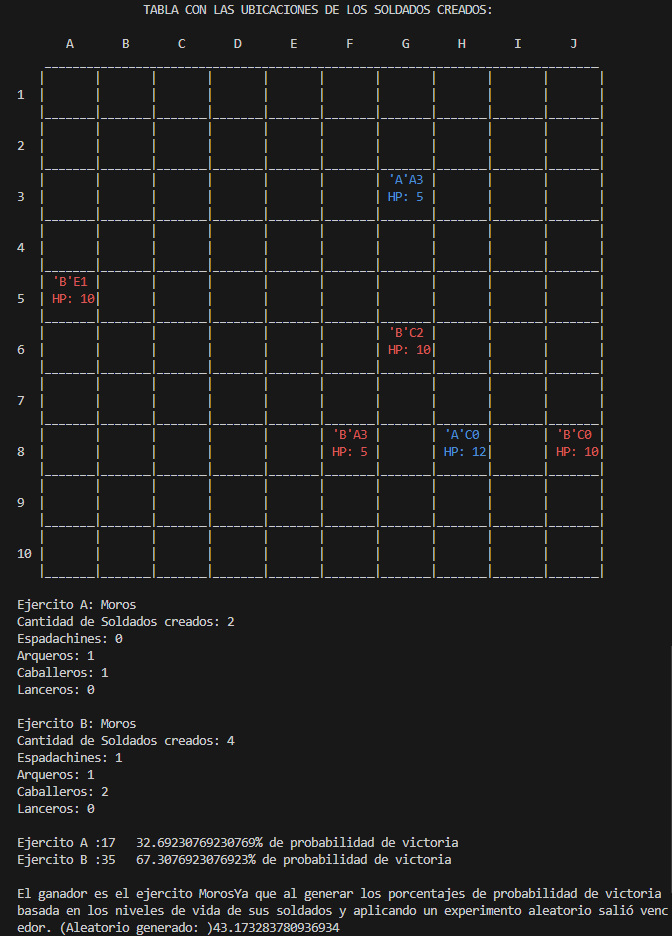
\includegraphics[width=1\textwidth,keepaspectratio]{img/showArmyTable.png}
    \caption{}
\end{figure}


\subsubsection{Método para mostrar datos generales del ejército respecto a los soldados}
\begin{itemize}
    \item El método tiene como nombre \textcolor{blue}{mostrarData()}.
    \item El método accede a los tipos de soldado de cada uno perteneciente al ejército seleccionado, utilizando un foreach va contabilizando cuantos soldados de cada tipo tiene dicho ejército.
    \item Finalizando muestra el resultado del conteo.
\end{itemize}
\lstinputlisting[language=Java, firstline=187, lastline=204,firstnumber=187,numbers=left]{src/VideoJuego7.java}


\subsubsection{Método para calcular las probabilidades de los ejércitos y mostrar un ganador}
\begin{itemize}
    \item El método tiene como nombre \textcolor{blue}{mostrarInfo()}.
    \item Siguiendo la métrica dada en las indicaciones se calcula la probabilidad de ser vencedores en cada ejército, mostrarlas y finalmente dar un ganador en base a las probabilidades realizadas.
\end{itemize}
\lstinputlisting[language=Java, firstline=206, lastline=230,firstnumber=206,numbers=left]{src/VideoJuego7.java}


\subsubsection{Método para mostrar los datos de los soldados de un ejército}
\begin{itemize}
    \item El método tiene como nombre \textcolor{blue}{showArmyData()}.
    \item Este usa un for each para recorrer el HashMap unidimensional de Soldado, y luego mostrar sus datos con el System.out.println, que a su vez este sigue el formato que se estableció en el método \textcolor{blue}{toString()} de la clase Soldado.java.
    \item La impresión en consola será la misma que la figura 1.
\end{itemize}
\lstinputlisting[language=Java, firstline=232, lastline=236,firstnumber=232,numbers=left]{src/VideoJuego7.java}




\subsubsection{Método para mostrar aquellos soldados con más vida de un ejército}
\begin{itemize}
    \item El método tiene como nombre \textcolor{blue}{moreHealt()}.
    \item Este recibe el HashMap con los soldados de un ejército, además de un char que indica el nombre del equipo.
    \item Primero recorre el HashMap unidimensional de soldados haciendo uso de un bucle for, de esta manera obtendrá el máximo de vida del ejército, el cual será almacenado en un entero maxHealth.
    \item Finalmente imprimirá aquellos soldados que tengan la vida igual a maxHealth, con un for y un if que controlará aquello.
    \item En la impresión se incluye el nombre del ejército antes de mostrar a los soldados.
\end{itemize}
\lstinputlisting[language=Java, firstline=238, lastline=249,firstnumber=238,numbers=left]{src/VideoJuego7.java}


\subsubsection{Método para hallar el promedio de vida en un ejército}
\begin{itemize}
    \item El método tiene como nombre \textcolor{blue}{averageHealth()}.
    \item De manera breve como el método, este retorna una división entre la suma de la vida del ejército, haciendo uso del método \textcolor{blue}{sumHealth()} y dividiendo entre el tamaño del ejército.
\end{itemize}
\lstinputlisting[language=Java, firstline=251, lastline=253,firstnumber=251,numbers=left]{src/VideoJuego7.java}


\subsubsection{Método para hallar la suma de vida en un ejército}
\begin{itemize} f
    \item El método tiene como nombre \textcolor{blue}{sumHealth()}.
    \item Se utiliza un entero inicializado en 0 para mientras que se recorre el HashMap unidimensional de Soldado con un bucle for each, este entero (sum) va almacenando la vida de todos los soldados.
    \item Finalmente se retorna el entero \textcolor{blue}{sum}.
\end{itemize}
\lstinputlisting[language=Java, firstline=255, lastline=260,firstnumber=255,numbers=left]{src/VideoJuego7.java}


\subsubsection{Método de ordenamiento InsertionSort}
\begin{itemize}
    \item El método tiene como nombre \textcolor{blue}{insertionSort()}.
    \item El método tiene como finalidad ordenar el HashMap unidimensional de Soldado haciendo uso del algoritmo InsertionSort, tomando en cuenta la vida de los soldados que contiene cada soldado de dicho HashMap. Este algoritmo se extrajo de Geeksforgeeks y fue adaptado a este proyecto.
    \item \href{https://www.geeksforgeeks.org/insertion-sort/}{https://www.geeksforgeeks.org/insertion-sort/}
    \item CONCLUSIONES:
    \begin{itemize}
        \item El algoritmo recorre el HashMap desde el segundo soldado hasta el último, considerando cada vez al soldado como una "llave" y compara su salud con la de los soldados anteriores.
        \item Los soldaos son recorridos hacia la derecha en el HashMap hasta que se encuentren en la posición correcta según la vida del soldado "llave" actual. 
        \item El algoritmo de ordenamiento por inserción es más eficiente que el burbuja, pero a pesar de ello su complejidad sigue siendo de O($n^2$).
    \end{itemize}
\end{itemize}
\lstinputlisting[language=Java, firstline=262, lastline=276,firstnumber=272,numbers=left]{src/VideoJuego7.java}


\subsubsection{Método para imprimir los soldados de un ejército, ordenados según su vida}
\begin{itemize}
    \item El método tiene como nombre \textcolor{blue}{printArmyHealth()}.
    \item Este método recibirá un HashMap unidimensional de Soldado (previamente ordenado), lo recorrerá usando un bucle for y mostrará los soldados, teniendo en cuenta que primero se mostrarán los de mayor vida hasta los de menor.
\end{itemize}
\lstinputlisting[language=Java, firstline=278, lastline=282,firstnumber=278,numbers=left]{src/VideoJuego7.java}


\subsubsection{Método para seleccionar el equipo a personalizar}
\begin{itemize}
    \item El método tiene como nombre \textcolor{blue}{customGame()}.
    \item Se muestra los equipos disponibles a modificar, luego se recibe un entero que será la elección del usuario.
    \item Usando condicionales se elige el método adecuado para la elección.
    \item Se valida la entrada y luego se hace llamado al método \textcolor{blue}{customGameArmy()} enviando los respectivos argumentos.
\end{itemize}
\lstinputlisting[language=Java, firstline=284, lastline=296,firstnumber=284,numbers=left]{src/VideoJuego7.java}
\begin{itemize}\begin{itemize}\item Un ejemplo de como se muestra en la siguiente imagen:
\end{itemize}\end{itemize}
\begin{figure}[H]
    \centering
    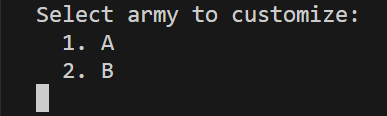
\includegraphics[width=0.5\textwidth,keepaspectratio]{img/12customGame.png}
    \caption{}
\end{figure}


\subsubsection{Método para mostrar la interfaz de juego personalizado}
\begin{itemize}
    \item El método tiene como nombre \textcolor{blue}{customGameArmy()}.
    \item Se muestra en pantalla las opciones y se recibe un entero valido que será la opción elegida por el usuario, para luego hacer un llamado al método correspondiente.
\end{itemize}
\lstinputlisting[language=Java, firstline=298, lastline=332,firstnumber=298,numbers=left]{src/VideoJuego7.java}

\newpage

\begin{itemize}\begin{itemize}\item Un ejemplo de como se muestra en la siguiente imagen:
\end{itemize}\end{itemize}
\begin{figure}[H]
    \centering
    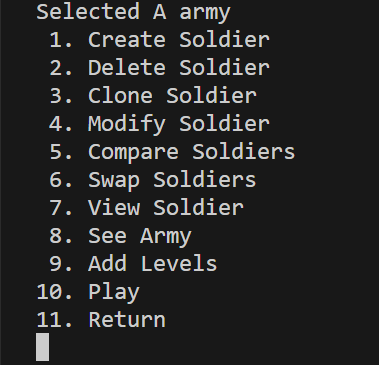
\includegraphics[width=0.5\textwidth,keepaspectratio]{img/12customGameArmy.png}
    \caption{}
\end{figure}


\subsubsection{Método para asignar los cambios realizados al ejercito elegido}
\begin{itemize}
    \item El método tiene como nombre \textcolor{blue}{assignModification()}.
    \item Se recibe el ejército personalizado y el char que contiene al equipo.
    \item Haciendo uso de una condicional se asigna al HashMap de clase del ejército correcto.
\end{itemize}
\lstinputlisting[language=Java, firstline=334, lastline=339,firstnumber=334,numbers=left]{src/VideoJuego7.java}

%\newpage

\subsubsection{Método para crear un soldado personalizado}
\begin{itemize}
    \item El método tiene como nombre \textcolor{blue}{createSoldier()}.
    \item En este método se recibe los datos del soldado a crear si el tamaño del ejército es menor a 10.
    \item Hace uso del método \textcolor{blue}{createPosition()} para los valores de la posición, en los demás casos los hace con el scanner y finalizada la recepción hace un llamado al segundo constructor.
\end{itemize}
\lstinputlisting[language=Java, firstline=341, lastline=363,firstnumber=341,numbers=left]{src/VideoJuego7.java}

\begin{itemize}\begin{itemize}\item Un ejemplo de como se muestra en la siguiente imagen:
\end{itemize}\end{itemize}
\begin{figure}[H]
    \centering
    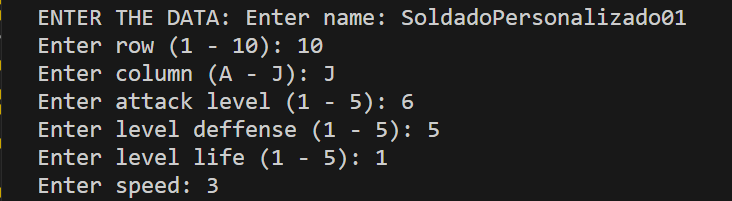
\includegraphics[width=0.8\textwidth,keepaspectratio]{img/12createSoldier.png}
    \caption{}
\end{figure}


\subsubsection{Método para crear una posición en el tablero}
\begin{itemize}
    \item El método tiene como nombre \textcolor{blue}{createPosition()}.
    \item El método recibe las coordenadas del soldado a crear y verifica que no esté ocupado, ya que en caso sea así este pedirá ingresar los datos nuevamente hasta que se ingrese un casillero vacío.
\end{itemize}
\lstinputlisting[language=Java, firstline=365, lastline=376,firstnumber=365,numbers=left]{src/VideoJuego7.java}


\subsubsection{Método para eliminar un soldado}
\begin{itemize}
    \item El método tiene como nombre \textcolor{blue}{deleteSoldier()}.
    \item Se muestra los soldados y luego se recibe el nombre del soldado a eliminar, se verifica que exista usando bucles y condicionales, en caso de que sí se eliminan del tablero principal y de l Hashmap de su equipo.
\end{itemize}
\lstinputlisting[language=Java, firstline=378, lastline=405,firstnumber=378,numbers=left]{src/VideoJuego7.java}

\begin{itemize}\begin{itemize}\item Un ejemplo de como se muestra en la siguiente imagen:
\end{itemize}\end{itemize}
\begin{figure}[H]
    \centering
    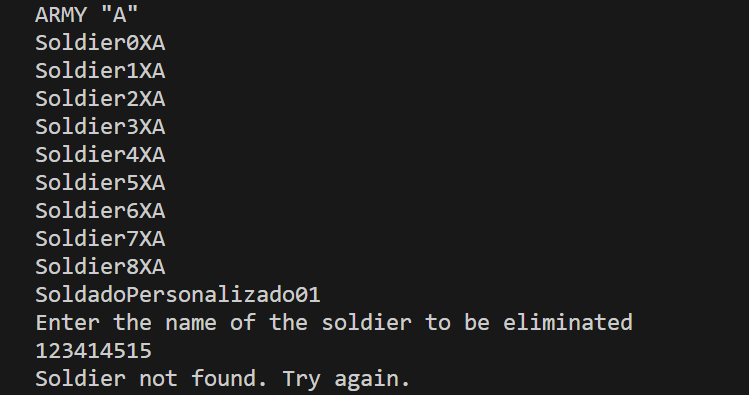
\includegraphics[width=0.6\textwidth,keepaspectratio]{img/12deleteSoldier.png}
    \caption{}
\end{figure}



\subsubsection{Método para clonar un soldado}
\begin{itemize}
    \item El método tiene como nombre \textcolor{blue}{cloneSoldier()}.
    \item Sigue la misma lógica de los métodos anteriores, solo que en este caso pide una posición para colocar el soldado clonado ya que no pueden haber 2 en la misma posición del tablero.
    \item En cuanto a lo demás realiza una copia de los atributos menos el del nombre ya que si se desearía utilizar en otro método no habría manera de saber a cual llamar.
\end{itemize}
\lstinputlisting[language=Java, firstline=407, lastline=446,firstnumber=407,numbers=left]{src/VideoJuego7.java}

\newpage

\begin{itemize}\begin{itemize}\item Un ejemplo de como se muestra en la siguiente imagen:
\end{itemize}\end{itemize}
\begin{figure}[H]
    \centering
    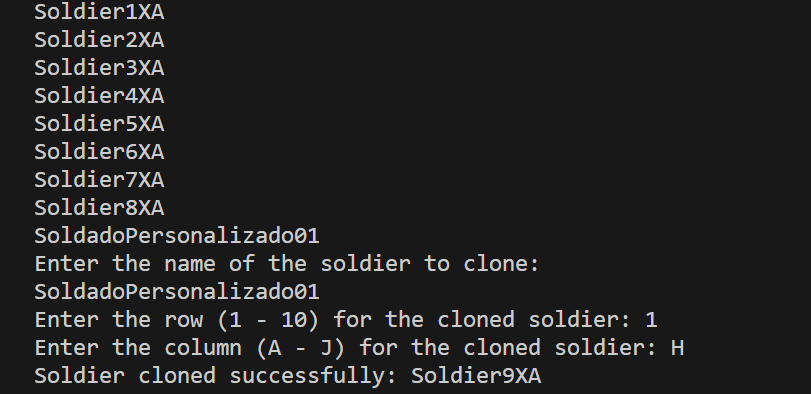
\includegraphics[width=0.65\textwidth,keepaspectratio]{img/12cloneSoldier.png}
    \caption{}
\end{figure}


\subsubsection{Método para modificar un soldado}
\begin{itemize}
    \item El método tiene como nombre \textcolor{blue}{modifySoldier()}.
    \item Primeramente se muestra el ejército y se solicita ingresar el nombre del soldado a modificar.
    \item Se verifica que exista y luego de ello se muestra las opciones a modificar, se recibe la elección y se usa un switch para cada opción.
    \item Por último solo se le asigna el nuevo valor recibido al soldado.
\end{itemize}
\lstinputlisting[language=Java, firstline=448, lastline=495,firstnumber=448,numbers=left]{src/VideoJuego7.java}

\begin{itemize}\begin{itemize}\item Un ejemplo de como se muestra en la siguiente imagen:
\end{itemize}\end{itemize}
\begin{figure}[H]
    \centering
    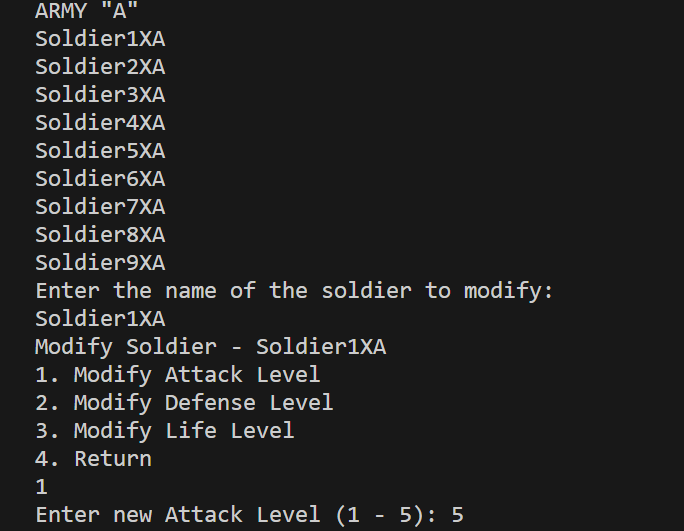
\includegraphics[width=0.65\textwidth,keepaspectratio]{img/12modifySoldier.png}
    \caption{}
\end{figure}

\newpage


\subsubsection{Método para comparar soldados}
\begin{itemize}
    \item El método tiene como nombre \textcolor{blue}{compareSoldiers()}.
    \item Pide los nombres de los dos soldados a comparar, para luego verificar que exista y posteriormente hacer uso del método \textcolor{blue}{compareSoldadoAttributes()} y con uso de condicionales mostrar si son idénticos o no.
\end{itemize}
\lstinputlisting[language=Java, firstline=497, lastline=520,firstnumber=497,numbers=left]{src/VideoJuego7.java}

\begin{itemize}\begin{itemize}\item Un ejemplo de como se muestra en la siguiente imagen:
\end{itemize}\end{itemize}
\begin{figure}[H]
    \centering
    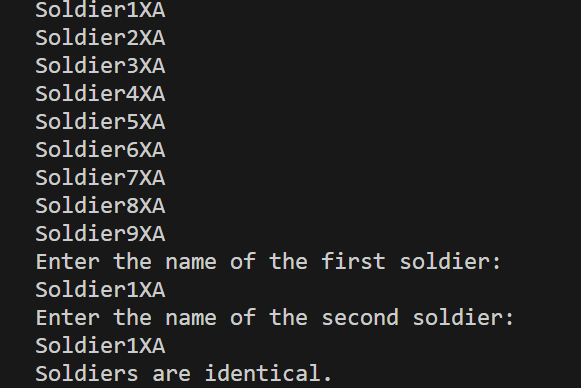
\includegraphics[width=0.65\textwidth,keepaspectratio]{img/12compareSoldiers.png}
    \caption{}
\end{figure}


\subsubsection{Método para buscar un soldado}
\begin{itemize}
    \item El método tiene como nombre \textcolor{blue}{findSoldado()}.
    \item Se envia el nombre del soldado como atributo junto a la estructura de datos que contiene su ejército, se usa un bucle for each para recorrer y retornar el soldado en caso exista.
\end{itemize}
\lstinputlisting[language=Java, firstline=522, lastline=527,firstnumber=522,numbers=left]{src/VideoJuego7.java}


\subsubsection{Método para comparar los atributos de un soldado}
\begin{itemize}
    \item El método tiene como nombre \textcolor{blue}{compareSoldadoAttributes()}.
    \item El método obtiene los atributos de ambos soldados y los compara dentro del mismo return.
\end{itemize}
\lstinputlisting[language=Java, firstline=529, lastline=535,firstnumber=529,numbers=left]{src/VideoJuego7.java}

\subsubsection{Método para intercambiar posiciones de 2 soldados}
\begin{itemize}
    \item El método tiene como nombre \textcolor{blue}{swapSoldiers()}.
    \item Muestra los soldados y luego recibe los nombres de los soldados a intercambiar verificando que existan.
    \item Posteriormente realiza las modificaciones tanto de sus atributos como en el tablero principal.
\end{itemize}
\lstinputlisting[language=Java, firstline=537, lastline=568,firstnumber=537,numbers=left]{src/VideoJuego7.java}

\begin{itemize}\begin{itemize}\item Un ejemplo de como se muestra en la siguiente imagen:
\end{itemize}\end{itemize}
\begin{figure}[H]
    \centering
    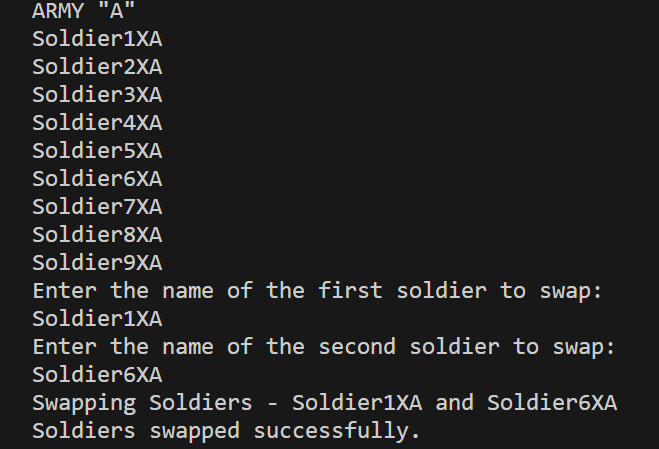
\includegraphics[width=0.65\textwidth,keepaspectratio]{img/12swapSoldiers.png}
    \caption{}
\end{figure}

\begin{lstlisting}[language=bash,caption={Commit \href{https://github.com/hernanchoquehuanca/fp2-23b/commit/e1a4207fd503551b8f3cb55473c173f8a6b60ccb}{e1a4207}: Concluyendo las peticiones requeridas en la clase VideoJuego7.java}][H]
 $ git add .
 $ git commit -m "Concluyendo las peticiones requeridas en la clase VideoJuego7.java"
 $ git push -u origin main
\end{lstlisting}

\newpage

\subsubsection{Método para ver los datos de un soldado}
\begin{itemize}
    \item El método tiene como nombre \textcolor{blue}{viewSoldier()}.
    \item Muestra los soldados y solicita el nombre del soldado que se desea mostrar datos. Luego se busca el soldado y finalmente se muestra sus atributos.
\end{itemize}
\lstinputlisting[language=Java, firstline=570, lastline=590,firstnumber=570,numbers=left]{src/VideoJuego7.java}

\begin{itemize}\begin{itemize}\item Un ejemplo de como se muestra en la siguiente imagen:
\end{itemize}\end{itemize}
\begin{figure}[H]
    \centering
    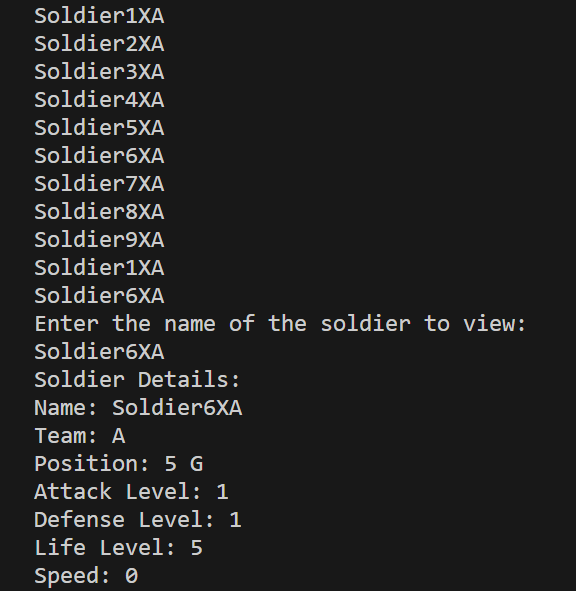
\includegraphics[width=0.45\textwidth,keepaspectratio]{img/12viewSoldier.png}
    \caption{}
\end{figure}


\subsubsection{Método para ver un ejército}
\begin{itemize}
    \item El método tiene como nombre \textcolor{blue}{seeArmy}.
    \item Sigue la misma lógica que el método anterior para ver soldados, de hecho podría reutilizarse para este método.
\end{itemize}
\lstinputlisting[language=Java, firstline=592, lastline=606,firstnumber=592,numbers=left]{src/VideoJuego7.java}


\subsubsection{Método para ver la sumatoria de niveles de un ejército}
\begin{itemize}
    \item El método tiene como nombre \textcolor{blue}{addLevels()}.
    \item El método usa un bucle for each para recorrer el ejército, luego va aumentando los valores de cada nivel de soldado para luego contenerlo en una variable entera y ser mostrada al final.
\end{itemize}
\lstinputlisting[language=Java, firstline=608, lastline=624,firstnumber=608,numbers=left]{src/VideoJuego7.java}

\begin{itemize}\begin{itemize}\item Un ejemplo de como se muestra en la siguiente imagen:
\end{itemize}\end{itemize}
\begin{figure}[H]
    \centering
    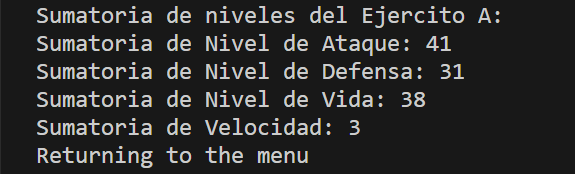
\includegraphics[width=0.6\textwidth,keepaspectratio]{img/12addLevels.png}
    \caption{}
\end{figure}


\subsubsection{Método para jugar ejército contra ejército}
\begin{itemize}
    \item El método tiene como nombre \textcolor{blue}{play()}.
    \item En este caso solo hace llamada al método \textcolor{blue}{gameInterfaz()}. que es la interfaz del juego 1v1.
\end{itemize}
\lstinputlisting[language=Java, firstline=626, lastline=628,firstnumber=626,numbers=left]{src/VideoJuego7.java}


\subsubsection{Método para mostrar al ejército ganador}
\begin{itemize}
    \item El método tiene como nombre \textcolor{blue}{amryWinner()}.
    \item Este método imprimirá al ejército ganador, usando como condición su tamaño.
    \item El método sólo será llamado cuando se verifique que uno de los dos ejércitos está vacío.
\end{itemize}
\lstinputlisting[language=Java, firstline=630, lastline=635,firstnumber=630,numbers=left]{src/VideoJuego7.java}


\subsubsection{Método para remover un soldado}
\begin{itemize}
    \item El método tiene como nombre \textcolor{blue}{removeSoldier()}.
    \item Obtiene el ejército al que pertenece y lo elimina tanto del HashMap de su ejército y del tablero de juego.
\end{itemize}
\lstinputlisting[language=Java, firstline=637, lastline=643,firstnumber=637,numbers=left]{src/VideoJuego7.java}


\subsubsection{Método para ejecutar la interfaz del juego}
\begin{itemize}
    \item El método tiene como nombre \textcolor{blue}{gameInterfaz()}.
    \item Se controla que el tamaño de los ejércitos no sea 0, de esta manera cuando lo sea se rompera el bucle while y se dará el nombre del ganador usando el método \textcolor{blue}{amryWinner()}.
\end{itemize}
\lstinputlisting[language=Java, firstline=645, lastline=661,firstnumber=645,numbers=left]{src/VideoJuego7.java}


\subsubsection{Método para la ejecución del turno del jugador}
\begin{itemize}
    \item El método tiene como nombre \textcolor{blue}{turn()}.
    \item Primero se comienza mostrando el tablero de juego. Luego se recibe las coordenadas del soldado a mover, para verificar se hace uso del método \textcolor{blue}{checkSoldier1()} y así llamar a \textcolor{blue}{turn2()}.
\end{itemize}
\lstinputlisting[language=Java, firstline=663, lastline=674,firstnumber=663,numbers=left]{src/VideoJuego7.java}

\newpage

\subsubsection{Método para revisar que el soldado elegido sea válido}
\begin{itemize}
    \item El método tiene como nombre \textcolor{blue}{checkSoldier1()}.
    \item Este fue utilizado en el método anterior, verifica que las coordenadas estén dentro del tablero y pertenezca al equipo del cual es turno.
\end{itemize}
\lstinputlisting[language=Java, firstline=676, lastline=688,firstnumber=676,numbers=left]{src/VideoJuego7.java}


\subsubsection{Método para analizar la posición a mover}
\begin{itemize}
    \item El método tiene como nombre \textcolor{blue}{checkSoldier2()}.
    \item Esta es la segunda verificación ya que evalúa si se va a producir un movimiento a un casillero libre, hay un enemigo o aliado. Luego de eso regresa el entero según sea el caso.
\end{itemize}
\lstinputlisting[language=Java, firstline=690, lastline=698,firstnumber=690,numbers=left]{src/VideoJuego7.java}

\newpage

\subsubsection{Método para ejecutar el movimiento elegido}
\begin{itemize}
    \item El método tiene como nombre \textcolor{blue}{turn2()}.
    \item Esté método recibe la coordenada a donde se desea mover el soldado que fue elegido previamente.
    \item Además de contener los posibles movimientos en caso sea válido, por ejemplo una pelea de soldados.
\end{itemize}
\lstinputlisting[language=Java, firstline=700, lastline=722,firstnumber=700,numbers=left]{src/VideoJuego7.java}


\subsubsection{Método para mover un soldado 1}
\begin{itemize}
    \item El método tiene como nombre \textcolor{blue}{moveSoldier()} y es sobrecargado.
    \item El método coloca el soldado en la posición previamente recibida y la remueve de su posición anterior.
\end{itemize}
\lstinputlisting[language=Java, firstline=724, lastline=727,firstnumber=724,numbers=left]{src/VideoJuego7.java}



\subsubsection{Método para mover un soldado 2}
\begin{itemize}
    \item El método tiene como nombre \textcolor{blue}{moveSoldier() y es sobrecargado}.
    \item Al contrario del método anterior este cuenta con parámetros distintos ya que incluye un soldado, pero realiza la misma función que el método anterior, pero este en caso de haber un soldado ganador de una pelea.
\end{itemize}
\lstinputlisting[language=Java, firstline=729, lastline=732,firstnumber=729,numbers=left]{src/VideoJuego7.java}


\subsubsection{Método para ejecutar la pelea de dos soldados}
\begin{itemize}
    \item El método tiene como nombre \textcolor{blue}{soldiersFight()}.
    \item Este método es uno de los más importantes ya que ejecuta la pelea entre dos soldados.
    \item Crea las probabilidades proporcionalmente a la suma de vida actual de ambos soldados.
    \item Muestra las probabilidades y luego elije de manera aleatoria con uso de Random de java.util, para finalmente mostrar al soldado ganador y llamar a los métodos necesarios que se encarguen de eliminar y mover los soldados según sea la situación.
\end{itemize}
\lstinputlisting[language=Java, firstline=734, lastline=756,firstnumber=734,numbers=left]{src/VideoJuego7.java}

\begin{lstlisting}[language=bash,caption={Commit \href{https://github.com/hernanchoquehuanca/fp2-23b/commit/0836847c1822bcc6dfa047a2a890ebfb3a5b8116}{0836847}: Versión final del código (lab20)}][H]
 $ git add .
 $ git commit -m "Ultimas modificaciones, version final del lab20"			
 $ git push -u origin main
\end{lstlisting}

     

%----------------------------- DIAGRAMA DE CLASE UML -------------------------------

\newpage

\subsection{Diagrama de clase UML}
\begin{figure}[H]
    \centering
    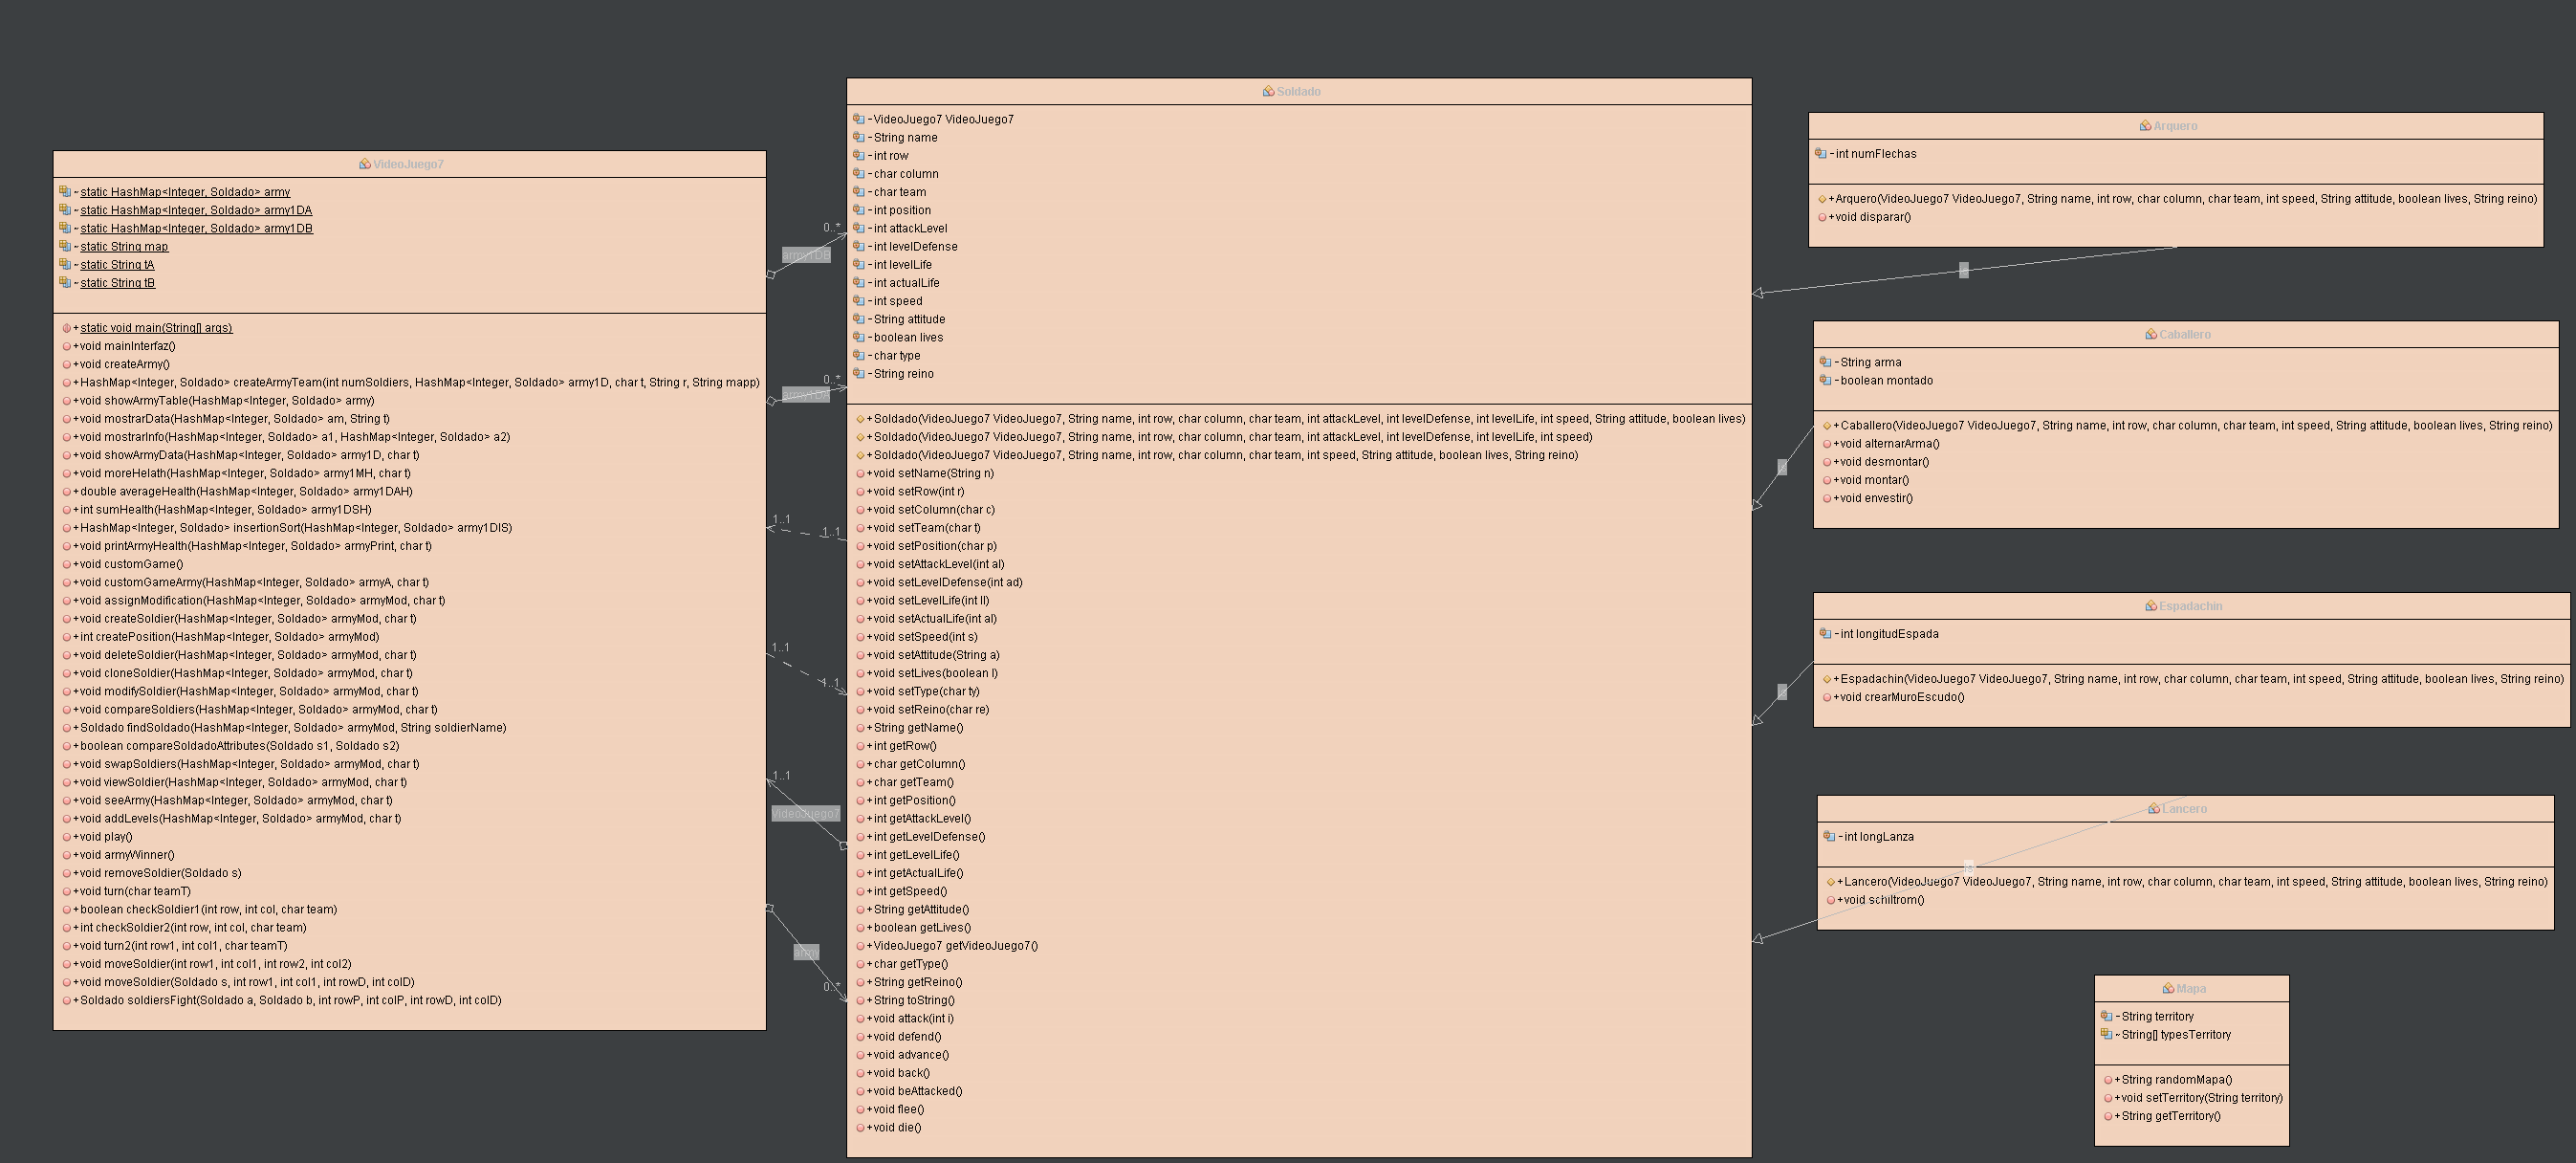
\includegraphics[width=1.1
    \textwidth,keepaspectratio]{img/20uml.png}
    \caption{}
\end{figure}

\href{https://github.com/hernanchoquehuanca/fp2-23b/blob/main/fase03/lab20/latex/img/20uml.png}{Diagrama 20 UML} para acceder al diagrama UML del repositorio y se observe con más claridad.

%------------------------------ ESTRUCTURA DE LABORATORIO --------------------------

\newpage

\subsection{Estructura de laboratorio \itemPracticeNumber} %%CAMBIAR NUMERO DE LAB
\begin{itemize}	
	\item El contenido que se entrega en este laboratorio es el siguiente:
\end{itemize}

%---------------------------------------- TREE -------------------------------------

\begin{lstlisting}[style=ascii-tree]

    lab20
    |   Soldado.java
    |   VideoJuego7.java
    |
    |───latex
        |   Informe_Lab20.pdf
        |   Informe_Lab20.tex
        |
        |───img
        |       12addLevels.png     
        |       12compareSoldiers.png  
        |       12customGame.png      
        |       12deleteSoldier.png  
        |       12swapSoldiers.png  
        |       12viewSoldier.png  
        |       logo_episunsa.png  
        |       mainInterfaz.png
        |       12cloneSoldier.png  
        |       12createSoldier.png    
        |       12customGameArmy.png  
        |       12modifySoldier.png  
        |       20uml.png           
        |       logo_abet.png      
        |       logo_unsa.jpg      
        |       showArmyTable.png
        |
        |───src
                Arquero.java
                Caballero.java
                Espadachin.java
                Lancero.java
                Mapa.java
                Soldado.java
                VideoJuego7.java

\end{lstlisting}    

\section{\textcolor{red}{Rúbricas}}
	
\subsection{\textcolor{red}{Entregable Informe}}
	\begin{table}[H]
		\caption{Tipo de Informe}
		\setlength{\tabcolsep}{0.5em} % for the horizontal padding
		{\renewcommand{\arraystretch}{1.5} % for the vertical padding
		\begin{tabular}{|p{3cm}|p{12cm}|}
			\hline
			\multicolumn{2}{|c|}{\textbf{\textcolor{red}{Informe}}}  \\
			\hline 
			\textbf{\textcolor{red}{Latex}} & \textcolor{blue}{El informe está en formato PDF desde Latex,  con un formato limpio (buena presentación) y fácil de leer.}   \\ 
			\hline 
		\end{tabular}
	}
	\end{table}
	
\clearpage

%------------------------------ RÚBRICA DE EVALUACIÓN ------------------------------
 
\subsection{\textcolor{red}{Rúbrica para el contenido del Informe y demostración}}
\begin{itemize}			
	\item El alumno debe marcar o dejar en blanco en celdas de la columna \textbf{Checklist} si cumplió con el ítem correspondiente.
	\item Si un alumno supera la fecha de entrega,  su calificación será sobre la nota mínima aprobada, siempre y cuando cumpla con todos lo ítem.
	\item El alumno debe auto calificarse en la columna \textbf{Estudiante} de acuerdo a la siguiente tabla:
	
    \begin{table}[ht]
    	\caption{Niveles de desempeño}
    	\begin{center}
    		\begin{tabular}{ccccc}
        	\hline
        	& \multicolumn{4}{c}{Nivel}\\
        	\cline{1-5}
        	\textbf{Puntos} & Insatisfactorio 25\%& En Proceso 50\% & Satisfactorio 75\% & Sobresaliente 100\%\\
        	\textbf{2.0}&0.5&1.0&1.5&2.0\\
        	\textbf{4.0}&1.0&2.0&3.0&4.0\\
        	\hline
    		\end{tabular}
    	\end{center}
    \end{table}	
\end{itemize}

%------------------------------------ EVALUACIÓN -----------------------------------

\begin{table}[H]
    \caption{Rúbrica para contenido del Informe y demostración}
    \setlength{\tabcolsep}{0.5em} % for the horizontal padding
    {\renewcommand{\arraystretch}{1.5}% for the vertical padding
    %\begin{center}
    \begin{tabular}{|p{2.7cm}|p{7cm}|x{1.3cm}|p{1.2cm}|p{1.5cm}|p{1.1cm}|}
        \hline
        \multicolumn{2}{|c|}{Contenido y demostración} & Puntos & Checklist & Estudiante & Profesor\\
        \hline
        \textbf{1. GitHub} & Hay enlace URL activo del directorio para el  laboratorio hacia su repositorio GitHub con código fuente terminado y fácil de revisar. &2 &X &2 & \\ 
        \hline
        \textbf{2. Commits} &  Hay capturas de pantalla de los commits más importantes con sus explicaciones detalladas. (El profesor puede preguntar para refrendar calificación). &4 &X &4 & \\ 
        \hline 
        \textbf{3. Código fuente} &  Hay porciones de código fuente importantes con numeración y explicaciones detalladas de sus funciones. &2 &X &2 & \\ 
        \hline 
        \textbf{4. Ejecución} & Se incluyen ejecuciones/pruebas del código fuente  explicadas gradualmente. &2 &X &2 & \\ 
        \hline			
        \textbf{5. Pregunta} & Se responde con completitud a la pregunta formulada en la tarea.  (El profesor puede preguntar para refrendar calificación).  &2 &X &2 & \\ 
        \hline	
        \textbf{6. Fechas} & Las fechas de modificación del código fuente están dentro de los plazos de fecha de entrega establecidos. &2 &X &2 & \\ 
        \hline 
        \textbf{7. Ortografía} & El documento no muestra errores ortográficos. &2 &X &2 & \\ 
        \hline 
        \textbf{8. Madurez} & El Informe muestra de manera general una evolución de la madurez del código fuente,  explicaciones puntuales pero precisas y un acabado impecable.   (El profesor puede preguntar para refrendar calificación).  &4 &X &3 & \\ 
        \hline
        \multicolumn{2}{|c|}{\textbf{Total}} &20 & &19 & \\ 
        \hline
    \end{tabular}
    %\end{center}
    %\label{tab:multicol}
    }
\end{table}
\clearpage

%------------------------------ REFERENCIAS ------------------------------

\section{Referencias}
\begin{itemize}			
    \item \url{https://docs.oracle.com/javase/tutorial/java/nutsandbolts/variables.html}
    \item \url{https://docs.oracle.com/javase/8/docs/api/java/util/HashMap.html}
    \item \url{https://docs.oracle.com/javase/tutorial/java/javaOO/methods.html}
    \item \url{https://www.geeksforgeeks.org/insertion-sort/}
    \item \url{https://es.stackoverflow.com/questions/108171/}
    \item \url{https://docs.oracle.com/javase/tutorial/java/IandI/subclasses.html}
    \item \url{https://docs.oracle.com/javase/tutorial/java/IandI/polymorphism.html}
\end{itemize}	
	
%\clearpage
%\bibliographystyle{apalike}
%\bibliographystyle{IEEEtranN}
%\bibliography{bibliography}
\end{document}